\chapter{Computational Model}
\label{chapter:computational_model}

In the following chapter we introduce the methods used for the numerical treatment of the governing equations
stated in the previous chapter.
We show that we can reformulate them in a succinct scheme which is able to resolve the dynamics of our system and allow
us to advance it in time.
At the end of this chapter we introduce an analytical test case that is used in Chapter \ref{chapter:results} to verify that the terms
emanating from the right-hand side term of Eq. \ref{eq:fokkerPlanckTerm} are correctly computed 
and show the expected convergence rate of our scheme.

\section{Field Solvers}
\label{section:field_solvers}

In this section we present the numerical methods to solve the elliptic \gls{pde}s introduced in the
previous chapter.
We introduce two solver types that are based on the Fast Fourier transform (\gls{fft})
and highlight their strengths and weaknesses.
Both methods aim to solve the electrostatic Poisson's equation (\ref{eq:poissonEquation}), or
equations that show similar structure w.r.t. the used differential operators.
Albeit their approach differs slightly, both methods impose open boundary (free-space)
conditions ($\lim_{\lVert \vect r \rVert_2 \to \infty} \phi(\vect r) = 0$).
Instead of using the above formulation of the \gls{pde} we opt to formulate it as a convolutional integral
using Green's function:

\begin{equation}
    \phi(\vect r) = \int G(\vect r - \vect r') \rho(\vect r') d \vect r',
    \label{eq:greenConvolution}
\end{equation}

where $G(\vect r) = -\frac{1}{4\pi r}$ is the analytical Green's function for the Poisson problem in 3
dimensions given open boundary conditions. 
Similarly, $G(\vect r) = \frac{r}{8 \pi}$ is its formulation for the biharmonic problem stated in Eq.
\ref{eq:diffusionCoeff}.
For their truncated spectral representations we direct the reader to Table 1 in \cite{vicoGreengard2016}.

The fact that Eq. \ref{eq:greenConvolution} is a convolution, gives us the ability to employ the
aforementioned Fast Fourier Transform.
Another advantage of this integral form is that we can readily compute the $\vect E(\vect r)$ field
by employing differentiation in Fourier space, maintaining the same accuracy as the method itself
without having to rely on an accurate finite difference stencil.

\subsubsection{Hockney-Eastwood}
\label{subsection:hockney}

The algorithm introduced by Hockney and Eastwood \cite{Hockney2021} (henceforth called Hockney's
method) extends the charge distribution $\rho(\vect r)$ by doubling the mesh along each spatial dimension.
In this newly added part of the mesh we set the values to zero. Albeit this allows us to 
use efficient cyclic convolution, it comes with a higher memory
footprint not only for the increased size of the charge distribution ($(2N)^d$), but also due to the
doubling of the domain for Green's function.

Due to the simple nature of this trick, it is easy to implement and also features good
computational complexity: $\mathcal{O}((2N)^d \log(2N)^d )$ and an error convergence of up to
$\mathcal O(N^{-2})$ \cite{zou2021fft}.

\subsubsection{Vico-Greengard}
\label{subsection:vico}

This comparatively new method, introduced in 2016 \cite{vicoGreengard2016} by Vico et al.
(henceforth called Vico's method), can be seen as a feasible alternative to the aforementioned Hockney method. 
Given sufficient smoothness of $\rho(\vect r)$, it shows spectral convergence: $\mathcal O(\gamma^N)$, where $\gamma \in (0,1)$.
Due to the oscillatory nature of the truncated Green's function it requires a mesh of $(4 N)^d$
(zero-padded as in Hockney's case). But luckily the authors showed that one can precompute the
Green's function on $(4N)^d$ in an initialization step and subsequently restricting it to $(2 N)^d$
without loosing accuracy in the solution.
Thus for a fixed Green's function, solving the actual Poisson equation uses at most as much 
memory as Hockney's method.

We must point out that the authors not only provide a formulation of Green's function for the
regular Poisson problem but also for several other commonly encountered \gls{pde}s, including the
biharmonic equation which we also make use of for solving Equation \ref{eq:diffusionCoeff}.

\section{Particle-in-Cell Method}
\label{section:PIC_method}

As explained in the previous chapter, we are interested in modeling the time evolution of the phase
space $f(\vect r,\vect v)$ in a single-species plasma. 
In Equation \ref{eq:fokkerPlanckTerm}, one of the dominating terms governing the dynamics of
the particles in such a plasma is defined by long-range interactions via the self-generated electric field.
\gls{pic} methods are one of the most efficient and widely used methods to
resolve such long-range interactions in areas of research such as fluid dynamics
\cite{evans1957particle,harlow1964pic}, astro physics and plasma physics \cite{bunemanPIC,dawson1971Plasma}.

Its strength lies in the ability to combine two traditional numerical techniques to describe the
flow of a field, known as the Eulerian and Lagrangian description.
\gls{pic} uses a computational mesh in combination with so called macroparticles, which are able to move
freely between the cells of the mesh according to Newton's equation of motion.
Meshes in a Eulerian system are suitable for resolving distortions in the medium but show an undesired diffusive
property in moving discontinuities. The Lagrangian particle view on the other hand, allows to properly
resolve the latter but shows deficiencies when strong distortions appear \cite{harlow1987picprogeny}.

In our case, the particles implicity represent the phase space distribution $f(\vect r,\vect v)$
and carry other macroscopic system properties important to our simulation.
We will now illustrate two common operations that are essential to the \gls{pic} algorithm.

\begin{figure}[h]
    \begin{center}
        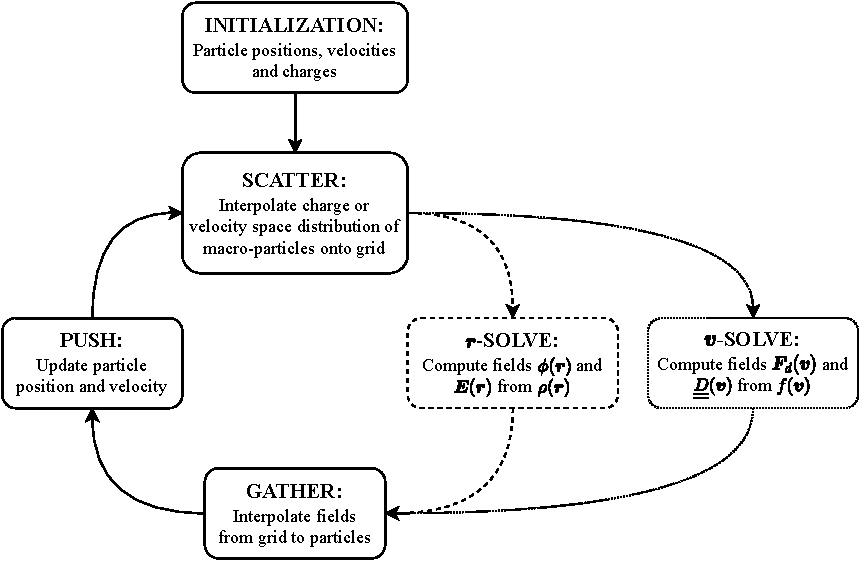
\includegraphics[width=0.88\textwidth]{figures/computational_model/PIC_loops_bw.pdf}
    \end{center}
    \caption{Flow chart of an extended PIC loop. The dashed lines depict the path for quantities computed in
    configuration space, whereas the dotted lines respresent the path for quantities computed in
velocity space.}
    \label{fig:PICloops}
\end{figure}

Given a charge density defined by the particle positions in configuration-space, we are interested
in solving the Poisson equation (cf. Eq. \ref{eq:poissonEquation}) with the \gls{pic} method and subsequently computing the interaction forces 
induced by the self-generated electric field $\vect E(\vect r)$.
Via the so called \textbf{\texttt{Scatter}} operation we distribute charges carried by
the particles that are part of one cell, to itself and neighboring cell values. This charge assignment is treated
in further detail in \cite{Hockney2021Chapter223}.
We can then solve for the electric potential $\phi(\vect r)$ and electric field $\vect E(\vect r)$ with any
common mesh-based method (i.e. \gls{fft} or \gls{fd} stencils).
The $\vect E(\vect r)$ field in this case, needs to be interpolated back 
(i.e. \textbf{\texttt{Gather}}) from cells to the particles in its immediate neighborhood in order
to add force contributions to their trajectory of motion.
In alternating these two steps we are then able to simulate how the system evolves over time.
% In the Langevin solver we also make use of the velocity space density $f(\vect v)$ as part of the
% PIC routine.
The Langevin solver will carry out similar operations to obtain quantities that are a function of
the velocity space distribution $f(\vect v)$.
The two possible PIC loops are depicted in Fig. \ref{fig:PICloops}.


\subsubsection{\gls{p3m}}

\begin{figure}
    \begin{center}
        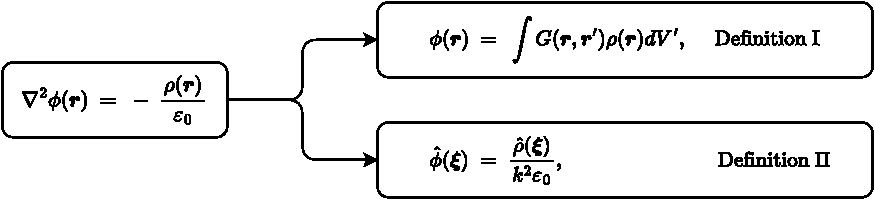
\includegraphics[width=0.88\textwidth]{figures/results/greenPoisson.pdf}
    \end{center}
    \caption{Two mathematically identical formulations of the solution to the Poisson problem
    \ref{eq:poissonEquation}. As used in Table \ref{table:langevinPossibleMethods}.}
    \label{fig:greenPoissonDefinitions}
\end{figure}

The \gls{p3m} method is an extension to the \gls{pic} scheme that additionally models \textbf{short-range} 
particle-particle (\gls{pp}) interactions. Hence the name (Particle-Particle)-(Particle-Mesh) method
(\gls{p3m}).
The method devised by Hockney and Eastwood \cite{Hockney2021} has gained popularity in settings
where we expect to encounter non-uniform particle distributions.
The \textbf{long-range} Particle-Mesh (\gls{pm}) forces acting on the particle's position in phase space are computed via solving
Poisson's equation with the \gls{pic} method (in Fourier space). This is identical to what we are doing in our collisionless solver.
The \textbf{short-range} \gls{pp}-interactions are computed in real-space by considering pairwise Coulomb interactions
with particles contained in a sphere of radius $r_c$ (chosen by the user).
This approach introduces a considerable computational cost as we have to do bookkeeping for storing
and updating the neighboring particles for each individual particle and quickly becomes infeasible
for larger cut-off radii or higher density plasma.
We direct the reader to \cite{Hockney2021} for a detailed discussion of the algorithmic details of the
\gls{p3m} algorithm.

\begin{table}[h]
    \renewcommand*\arraystretch{1.5}
    \centering
    \caption{Overview of explored  methods for the various quantities needed by the Langevin solver.}
    \label{table:langevinPossibleMethods}
    \begin{tabular}{|l|l|l|}
\hline
\textbf{\gls{pic} Type}                           & \textbf{Quantity of Interest}
                                            & \textbf{Comp. Domain or Method}     \\ \hline
\multirow{4}{*}{Electrostatic \gls{pic}} & \multirow{2}{*}{$\phi(\vect r)$}
                                         & Definition I (see Fig. \ref{fig:greenPoissonDefinitions})  \\ \cline{3-3} 
                                   &
                                   & Definition II (see Fig. \ref{fig:greenPoissonDefinitions})  \\ \cline{2-3} 
                                   & \multirow{2}{*}{$- \posNabla \phi(\vect r)$}
                                   & Finite Difference Gradient: $\fdPosNabla$ \\ \cline{3-3} 
                                   &
                                   & Spectral Gradient: $\spPosNabla$          \\ \hline
\multirow{4}{*}{Velocity \gls{pic}}      & \multirow{2}{*}{$\velNabla h(\vect v)$, $g(\vect v)$}
                                   & Hockney, $ \velNabla^{\{\text{fd,sp}\}} $                      \\ \cline{3-3} 
                                   &
                                   & Vico, $ \velNabla^{\{\text{fd,sp}\}} $                      \\ \cline{2-3} 
                                   & \multirow{2}{*}{$\frac{\partial^2}{\partial \vect v \partial
\vect v} g(\vect v)$} & Finite Difference Hessian: $\fdVelHess$ \\ \cline{3-3} 
                                   &
                                   & Spectral Hessian: $\spVelHess$           \\
\hline
\end{tabular}
\end{table}


\subsection{Methods Overview}

We have access to a \gls{p3m} solver by Ulmer \cite{p3m_ulmer} and can therefore readily 
apply it to the \gls{dih} problem to observe short-range interactions in the force
computation impacts the normalized emittance.
One crucial difference of Ulmer's collisionless solver to ours is, that he uses a Green's function 
directly defined in real space (see Definition I in Figure \ref{fig:greenPoissonDefinitions}) to
compute the potential $\phi$.
Whereas we define it via the integral formulation in Fourier space (Definition II).
Although these two formulations are mathematically identical under the periodicity assumption, 
we will observe two quite different outcomes in the normalized emittance.
Ulmer defines the Green's function as:

\begin{equation}
    G(\vect r, \vect r') = \frac{1}{4\pi \vp} \frac{\erf{(\alpha |\vect r -
    \vect r'|)}}{|\vect r - \vect r'|},
    \label{eq:greenPoissonDefinitions}
\end{equation}

where $\alpha= 1 \times 10^6$ is a parameter indicating the splitting of interactions into the
\gls{pm} and \gls{pp} parts.
Subsequently, we refer to a Langevin solver instance implementing Definition I as \emph{Langevin-I} and analogously \emph{Langevin-II} for an
instance employing Definition II.

So far we introduced a variety of building blocks we can use for the Langevin solver. Thus, it might
be difficult for the reader to follow the subsequently tested solver combinations.
In Table \ref{table:langevinPossibleMethods} we collect all the methods of computation
we explored for each quantity of interest (QoI) we need as part of our Langevin solver.

\section{Discretization of the Rosenbluth Potentials}
\label{section:rb_discretization}

After having derived expressions for both Rosenbluth potentials in Section
\ref{section:rb_potentials}, we now show how we compute them numerically.
As the name already suggests, they can be treated as potentials, similarly to what we would 
encounter computing an electric field defined by distributed particle charges (see Equations
\ref{eq:rbFirstPotential} and \ref{eq:rbSecondPotential}).

We have already touched upon the fact that it is a reasonable assumption to solve them in velocity space exclusively.
Since we expect our distribution to behave as $\lim_{\lVert \vect v \rVert_2 \to \infty} \int f(\vect r,
\vect v) d\vect r = 0$ \cite{hinton1983collisional}, the open-boundary solvers as introduced
in Section \ref{section:field_solvers} may be used here.

The friction and diffusion coefficients are readily computed from the potentials either by directly
differentiating them in Fourier space (see \cite{johnson2011FFTdifferentialtion}) or using a second
order centered finite difference stencil.
It has to be noted that the \gls{fd} approach would not satisfy the limit $\lim_{\lVert \vect v \rVert_2 \to \infty}
g(\vect v) = 0$ (as to the argument of Hinton \cite{hinton1983collisional}).

\subsubsection{Composable Finite Difference Operators}

In a situation where it is necessary to respect these boundary conditions with a \gls{fd}
stencil, one could explore one-sided stencils along the dimension with open boundary conditions.
We implemented a general interface for composing user defined stencils along either dimension
which are generated at compile time.
This allows us to define more complex operator structures such as the Hessian.
Further details on this tool with additional convergence studies can be found in Appendix 
\ref{appendix:chainable_operators}.
Although, as we will show with numerical experiments in Chapter \ref{chapter:results}, there is no
need for such a flexible operator.
The potential $g(\vect v)$ is indeed vanishingly small at the mesh boundaries given the properties of
the \gls{dih} problem (see Section \ref{section:dihProblem}).

After computing the coefficients on the grid, we scatter their values onto the macroparticles. This
way, we can use them directly in the time integrator described in the next section.

\subsection{Stochastic Description}
\label{sub:stochastic_description}

In Chapter \ref{section:focker_planck} we discussed how collisions can be thought of as a
Markov process where a particle experiences a small change in velocity due to many weak 
Coulomb collisions with other particles passing through its Debye sphere.
This derivation lead us to a formulation of the right-hand side of the Vlasov Equation
\ref{eq:vlasovEquation} containing a dynamic friction $\vect F_d$ and diffusion coefficient $\matr
D$ based on the Langevin equation.
The coefficients themselves are approximated with the help of the Rosenbluth potentials.

Based on these calculations, Risken \cite{Risken1984FokkerPlanckE} formulates the time evolution of
the Vlasov-Poisson-Fokker-Planck (\gls{vpfp}) equation as the following system of coupled differential equations
governing the motion of the macroparticles in the \gls{pic} approach:

\begin{equation}
\label{eq:SDE_system}
% \left\{  
% \begin{aligned}
%     \frac{\partial \vect r }{\partial t} &= \vect v \\
%     \frac{\partial \vect v}{\partial t} &= \frac{(\vect F_{mf} + \vect F_{ext})}{m} + \vect F_d + \matr Q \cdot d\vect W(t)^T.
% \end{aligned}
% \right.
\left\{  
\begin{aligned}
    d\vect r &= d\vect v dt, \\
    d \vect v &=  \frac{(\vect F_{mf} +\vect F_{ext})}{m} dt + \vect F_d dt + \matr Q \cdot d\vect W(t)^T.
\end{aligned}
\right.
\end{equation}


\subsubsection{Diffusion Matrix Factorization}
In Section \ref{section:focker_planck} we have listed an important property which we can now 
use to determine an appropriate factorization of $\matr D$.
We know that $\matr D$ is at least semi-positive definite \cite{stoel}. Thus, one feasible
algorithm would be the \gls{ldlt} factorization, which has the advantage that we can avoid computing
square-roots on the immediate matrix entries of $\matr D$ \cite{krishnamoorthy2013cholesky}.
This means we can factorize $\matr D = \matr L \matr S^2 \matr L^T$ such that $\matr Q = \matr S \matr L^T$ with
$\matr S$ being a diagonal matrix. See Appendix \ref{appendix:LDLT} for the details on how to compute
$\matr Q$ from $\matr L$ and $\matr S$.
We point out that the default Cholesky factorization would not be suitable, as for this
method to work, the matrix has to be positive definite.

\section{Resulting Scheme}
\label{section:resulting_scheme}

We have now successfully brought the \gls{vpfp} equation into a form that we can start thinking about an appropriate
timestepping scheme.
We opt for a simple but frequently used timestepping scheme that facilitates the Stochastic
Differential Equation (\gls{sde}) form of
our coupled system of Equations \ref{eq:SDE_system}.
It is based on the Euler-Maruyama scheme in conjunction with integrator splitting:

\begin{algorithm}
\caption{Time Integrator Procedure}
\label{alg:integrator}
\begin{algorithmic}[1]
\Procedure{Advance Particles in time by $dt$}{}
\State $\vect r \gets \vect r + \frac{dt}{2} \vect v$;
\State Compute $\vect F(\vect r)$; $\vect v \gets \vect v +  \frac{dt}{2} \frac{\vect F}{m}$;
\hfill\COMMENT{(Electrostatic PIC)}
\State Compute $\vect F_d(\vect v)$ and $\matr D(\vect v)$; \hfill\COMMENT{(Velocity PIC)}
\State Factorize $\matr D(\vect v)$; $\matr Q \gets \matr S \matr L^T$; \hfill\COMMENT{(Cholesky
Factorization)}
\State $\vect v \gets \vect v + dt \vect F_d + d\vect W(t) \cdot \matr Q$;
\State Compute $\vect F(\vect r)$; $\vect v \gets \vect v + \frac{dt}{2} \frac{\vect F}{m}$;\hfill\COMMENT{(Electrostatic PIC)}
\State $\vect r \gets \vect r + \frac{dt}{2} \vect v$;
\EndProcedure.
\end{algorithmic}
\end{algorithm}

We have chosen this scheme as it has been shown to work well for integrating the \gls{vpfp} equation,
albeit in a different setting \cite{stoel}.
It exhibits a symmetric update structure w.r.t. step 4 through 6. This would enable subcycling
on the collisional terms if necessary (similar to Adam \cite{subcyclingAdam1982}).

\subsubsection{Boundary Conditions}

When solving \gls{pde}s, boundary conditions are of utmost importance for achieving uniqueness and
physical correctness. In our problem setting we solve the \gls{pde}s arising from the \gls{fp} equation
in velocity phase space with open boundaries.
For the computation of the self-generated electric field we choose periodic boundary conditions.
This was mainly chosen to facilitate a direct comparison to Ulmer's results \cite{p3m_ulmer} (see
Section \ref{section:simulation_setup}).

\subsection{Advantages over \gls{p3m}}
Having introduced all important parts of the Langevin method, we can elaborate on the advantages 
it brings compared to the \gls{p3m} method.
The user of the \gls{p3m} method by Ulmer needs to set two hyperparameters: $\alpha$, defining
the splitting ratio of Green's function interaction potential into a long-range and short-range
part, as well as the cut-off radius $r_c$ which defines the range of the \gls{pp} collisions. Although not
strictly a hyperparameter but still impactful, there exist a multitude of charge-shaping functions
to choose from (i.e. Gaussian, polynomials).
This can make it a delicate endeavor to properly tune the method for a certain problem.

The Langevin method on the other hand regulates the effect of collision by choosing the Coulomb
logarithm $\ln \Lambda$.
It is used in the derivation of the \gls{fp} coefficients for defining a cut-off for weak
Coulomb interactions at large impact parameters. Thus, in a sense it serves a similar purpose as 
$r_c$ in the \gls{p3m} method.
Depending on the state of plasma one can choose its magnitude appropriately as it is
dependent on the system's temperature.

\subsubsection{Computational Complexity}
The computational complexity is an important criterion to understand in what cases one algorithm
might be superior to another.
The Langevin approach significantly improves upon the computational complexity of the
\gls{p3m} method.

For \gls{p3m} it can be split up into the \gls{pp} and the \gls{pm} part:
\begin{equation}
    C_{\text{\gls{p3m}}}(N_p, N_m, \delta) = \underbrace{\mathcal O( N_p^2 \delta^3)}_{\text{Particle-Particle}}
    + \underbrace{\mathcal O(N_p) 
    + \mathcal O(N_m \log(N_m))}_{\text{Particle-Mesh}},
\end{equation}
with $\delta = r_c / L$ for a uniform charge, where $r_c$ is the cut-off radius for short-range
interactions and $L$ is the domain length.
The $\mathcal O(N_p)$ term accounts for the scatter/gather operations.

The \gls{pm} term is also present in the Langevin method, while the term for the particle
particle interaction changes due to the computation of the \gls{fp} coefficients.
When omitting constant coefficients, it is asymptotically almost identical to the 
regular \gls{pic} solver, with the exception of the added $\mathcal O(N_m)$ term for the decomposition of the diffusion
coefficients $\matr D(\vect v)$ used in the time integrator:
\begin{align}
    \nonumber
    C_{\text{Langevin}}(N_p, N_m) &= \underbrace{\mathcal O(N_p) + \mathcal O(N_m \log(N_m))}_{\text{$\vect F_d$}} \\ \nonumber
                                          &+ \underbrace{\mathcal O(N_p) + \mathcal O(N_m) +
                                          \mathcal O(N_m \log(N_m))}_{\text{$\matr D$}} \\ \nonumber
                                          &+ \underbrace{\mathcal O(N_p) + \mathcal O(N_m \log(N_m))}_{\text{Particle-Mesh}} \\
    &= \mathcal O(N_p) + \mathcal O(N_m \log(N_m)). 
\end{align}

\section{Test Cases}
\label{section:test_cases}

To evaluate the correctness of our implementation we use simple initial conditions to which we know
the analytical solution of the potentials and coefficients discussed in Chapter \ref{chapter:background}.
This also gives us the ability to carry out studies on the error convergence with respect to a decreasing mesh width.

\subsubsection{Rate of Convergence}

When evaluating the performance of numerical methods, an important criterion is determine
the rate of convergence.
With this we mean how much better of an approximation we can expect to obtain when increasing the
discretization level (i.e. number of grid points) our method uses.
There exist two types of convergence we will encounter in Chapter \ref{chapter:results}.
We illustrate their asymptotic behavior on the example of the relative approximation error $\eta$ with increasing grid points $N_o$ (see Table \ref{table:nomenclature}):

\begin{align}
    \label{eq:convergenceDefinition}
    \eta(x, x_{\text{appr}}) &= \mathcal O(N_o^{-r}), \quad \quad \text{algebraic convergence with
    rate}\ r, \\
    \eta(x, x_{\text{appr}}) &= \mathcal O(\gamma^{N_o}), \quad \quad\ \text{exponential convergence
    with}\ \gamma
    \in (0,1),
\end{align}

where $x$ denotes the ground truth value (i.e. the analytical solution) and $x_{\text{appr}}$ the
approximation given by the applied numerical method.


\subsection{Centered Gaussian}
\label{sub:centered_gaussian}

We use a centered Gaussian probability density function with curvature $\sigma$ as our starting
point to emulate the phase space density $f(\vect v)$ in three-dimensional velocity space.
Each grid point in this space is associated with a Cartesian velocity vector $\vect{v} = \left [ v_x, v_y, v_z \right]^T$ and a respective euclidean norm $v  = \lVert \vect v \rVert_2 = \sqrt{v_x^2+v_y^2+v_z^2}$.
The resulting density is then described as
\begin{equation}
\label{eq:gaussian_pdf}
f(\vect{v}) = \frac{1}{\sqrt{8\pi^3} \sigma^3} \exp(-\frac{v^2}{2 \sigma^2}).
\end{equation}

The potentials by Rosenbluth (Eq. \ref{eq:rbFirstPotential} and Eq. \ref{eq:rbSecondPotential}), as
well as their derivatives, can be analytically derived and are listed in Equations \ref{eq:gaussian_sols}.
In the following formulation of the solutions we have already accounted for the prefactor of $8\pi$
that appears in Eqs. \ref{eq:rbFirstPotential} and \ref{eq:rbSecondPotential}.
They reflect what has been implemented in the computer code for this test case:

\begin{subequations}
\label{eq:gaussian_sols}
\begin{align}
    \begin{split}
    h(\vect v)                &= \frac{2}{v} \text{erf}\left( \frac{v}{\sqrt{2} \sigma} \right)
    \end{split}
    \eqVspace
    \begin{split}
    g(\vect v)                &= \sigma \sqrt{\frac{2}{\pi}} \exp(- \frac{v^2}{2 \sigma^2}) +
    \left(v + \frac{\sigma^2}{v}\right) \text{erf}\left( \frac{v}{\sqrt{2}\sigma} \right)
    \end{split}
    \eqVspace
    \begin{split}
    \nabla h(\vect v)         &= \left [ \sqrt{\frac{2}{\pi}} \frac{1}{\sigma} \exp(- \frac{v^2}{2
    \sigma^2}) - \frac{1}{v} \text{erf} \left( \frac{v}{\sqrt{2} \sigma} \right) \right ]  \vect v
    \end{split}
    \eqVspace
    \begin{split}
    \matr D_{i,i}(\vect v) &= \Gamma \sqrt{\frac{2}{\pi}} \frac{1}{\sigma} \exp(-\frac{v^2}{2 \sigma^2}) \\
                        & \quad \left[ \frac{\vect v_i - \sigma^2}{\sigma^2} + \frac{(\sigma^2 /
                        v + v) (\sigma^2 v^2 - \vect v_i^2 v^2 - \sigma^2
                \vect v_i^2)}{\sigma^2 v^3} + \frac{2 \vect v_i^2}{r^4}(v^2 - \sigma^2) \right] \\ 
                        & \quad + \frac{1}{v^5} \text{erf}\left( \frac{v}{\sqrt{2}\sigma} \right)
                        \left[ v^4 - v^2(\vect v_i^2 + \sigma^2) + 3 \sigma^2 \vect v_i^2
                        \right], \quad \forall i \in [1,3]
    \end{split}
    \eqVspace
    \begin{split}
        \matr D_{i,j}(\vect v)  &= \Gamma \left[ \left( \frac{3\sigma^2}{v^2} - 1 \right)
    \frac{\vect v_i \vect v_j}{v^3}\ \text{erf} \left( \frac{v}{\sqrt{2} \sigma} \right) - 3\sigma
\sqrt{\frac{2}{\pi}} \frac{\vect v_i \vect v_j}{v^4} \exp(- \frac{v^2}{2 \sigma^2}) \right],
\ \forall i \neq j.
    \end{split}
\end{align}
\end{subequations}

\subsubsection{Maxwellian}
\label{sub:maxwellian}

Multiplying Eq. \ref{eq:gaussian_pdf} with the number density $n_0$ and choosing $\sigma = v_{th}$, we obtain a centered Maxwellian distribution.
As we expect the velocity distribution function to relax to a Maxwellian
equilibrium distribution, it equips us with another important test case that closer resembles the
problem at hand, which is the disorder induced heating of a cold electron sphere (cf. Chapter 3.2.4.2 in Callen \cite{Callen}).
